\(\pagebreak\)

\section{List of Symbols}\label{list-of-symbols}

\section{Introduction}\label{introduction}

We propose a solution to a classic two-tank mixing liquids problem. The
liquids in this case are saline and pure water. The system consists of
two 100 L interconnected tanks which are referred to as Tank A and Tank
B. \(\autoref{fig:sys_illus}\) illustrates the setup of the tanks and
connections between them and an external system that feeds and drains
saltwater from both tanks

\begin{figure}
\centering
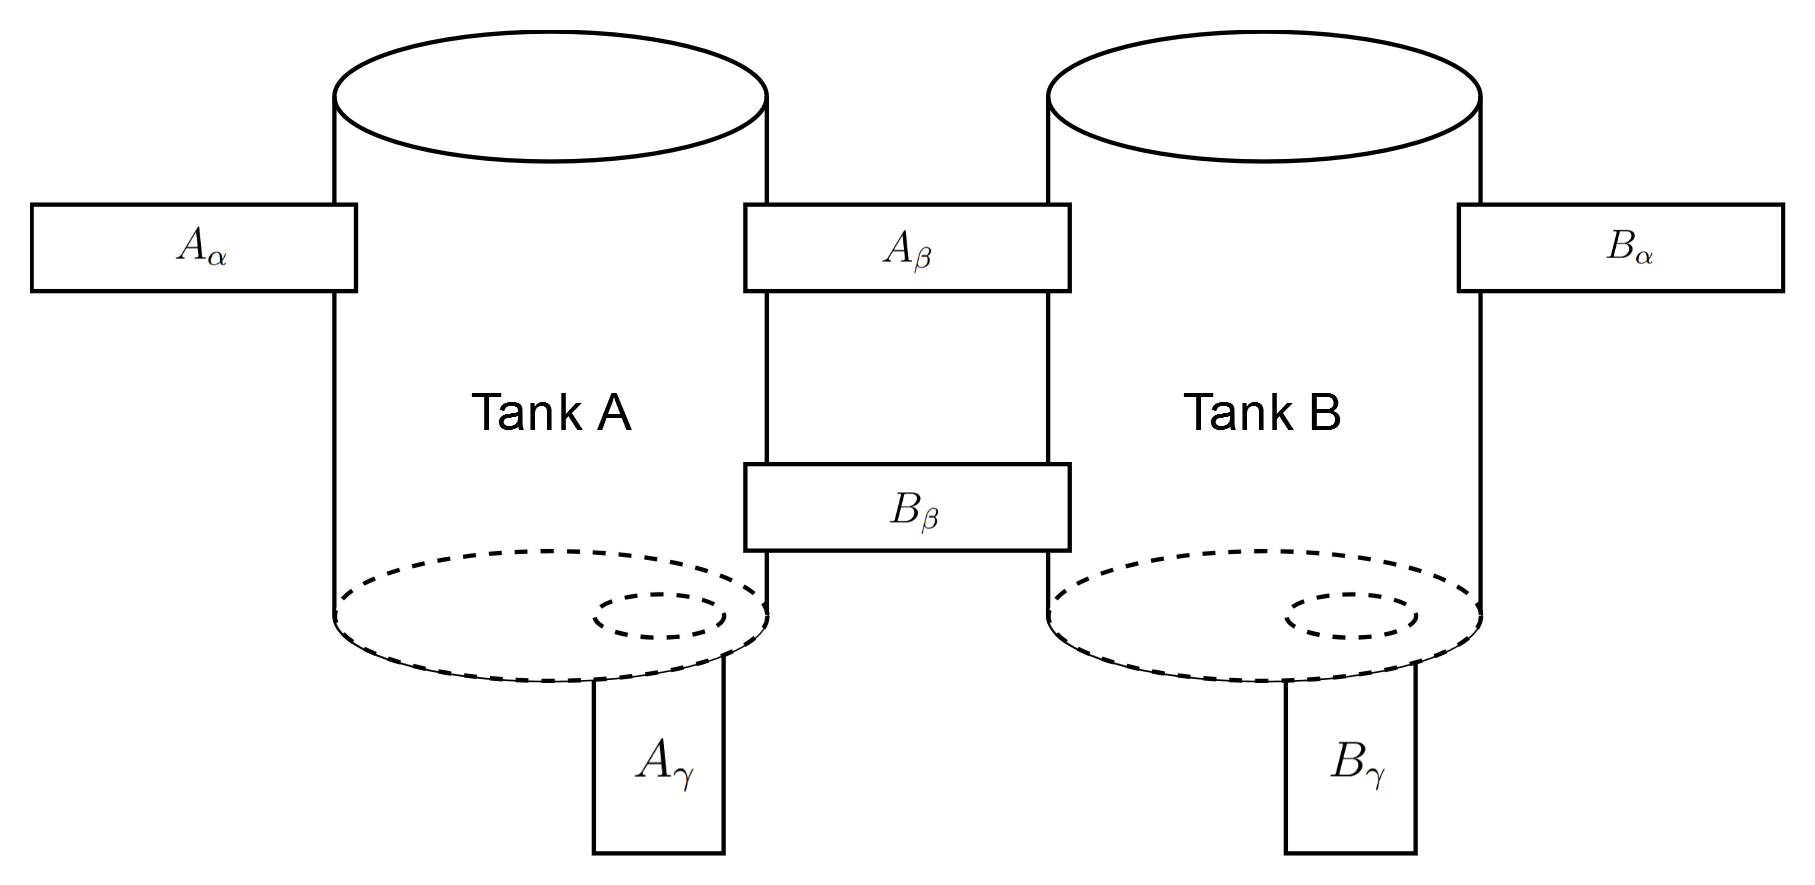
\includegraphics[width=0.75\linewidth,height=\textheight,keepaspectratio]{./mixing_tanks.png}
\caption{An illustration of the two-tank system}\label{fig:sys_illus}
\end{figure}

Each tank has four pipes connected to it. For Tank A, the pipe labelled
as \(A_\alpha\) delivers water with a salt concentration of \(K_A\) at a
rate of \(V_{A+}\). The two pipes labelled \(A_\beta\) and \(A_\gamma\)
drain water from Tank A into Tank B at a rate of \(V_{AB}\) and into the
external environment at \(V_{A-}\) respectively. Finally, the pipe
\(B_\beta\) delivers salt water from Tank B to Tank A at a rate of
\(V_{BA}\). The setup is the same for Tank B only that the symbols \(A\)
and \(B\) are interchanged in the parameters of Tank A to get those of
Tank B. \(\autoref{tab:flow_params}\) summarizes inflow and outflow
parameters for both tanks.

\begin{longtable}[]{@{}
  >{\raggedright\arraybackslash}p{(\linewidth - 6\tabcolsep) * \real{0.0800}}
  >{\centering\arraybackslash}p{(\linewidth - 6\tabcolsep) * \real{0.4400}}
  >{\centering\arraybackslash}p{(\linewidth - 6\tabcolsep) * \real{0.2533}}
  >{\centering\arraybackslash}p{(\linewidth - 6\tabcolsep) * \real{0.2267}}@{}}
\caption{Flow parameters and initial salt contents of both tanks.
\(\label{tab:flow_params}\)}\tabularnewline
\toprule\noalign{}
\begin{minipage}[b]{\linewidth}\raggedright
\end{minipage} & \begin{minipage}[b]{\linewidth}\centering
Inflow
\end{minipage} & \begin{minipage}[b]{\linewidth}\centering
Outflow
\end{minipage} & \begin{minipage}[b]{\linewidth}\centering
Initial salt mass
\end{minipage} \\
\midrule\noalign{}
\endfirsthead
\toprule\noalign{}
\begin{minipage}[b]{\linewidth}\raggedright
\end{minipage} & \begin{minipage}[b]{\linewidth}\centering
Inflow
\end{minipage} & \begin{minipage}[b]{\linewidth}\centering
Outflow
\end{minipage} & \begin{minipage}[b]{\linewidth}\centering
Initial salt mass
\end{minipage} \\
\midrule\noalign{}
\endhead
\bottomrule\noalign{}
\endlastfoot
Tank A & \(V_{A+}\) (\(K_A\) conc.), \(V_{BA}\) & \(V_{A-}\), \(V_{AB}\)
& 0 kg \\
Tank B & \(V_{B+}\) (\(K_B\) conc.), \(V_{AB}\) & \(V_{B-}\), \(V_{BA}\)
& 1 kg \\
\end{longtable}

At time \(t=0\), the initial salt concentrations in each tank are known,
and the system evolves dynamically according to the flow rates and
concentrations. The objective is to determine the steady-state salt
concentrations in each tank, as well as to analyze how the system
evolves under various parameter choices.

\section{Model}\label{model}

We base our model chiefly on the principle of conservation of mass. That
is, the rate of change of salt in each tank is equal to the difference
between the rate at which salt enters the tank and the rate at which it
leaves.

Let \(S_A(t)\) and \(S_B(t)\) represent the salt concentrations in Tanks
A and B respectively at time \(t\). The total mass of salt in each tank
at any time is given by the product of the concentration and the tank
volume. This follows from the constraint that the volumes in the tanks
remain constant, which can be ensured by choosing the right values for
the flow rate parameters. Also, we know from dimensional analysis that
the rate at which salt enters or leaves a tank is the product of the
flow rate and the concentration.

\subsection{Tank A Equation}\label{tank-a-equation}

Each of the four pipes connected to Tank A contribute a term to its
differential equation. We designate inflows as positive terms and
outflows as negative. \(A_\alpha\) and \(B_\beta\) are inflow pipes
while \(A_\beta\) and \(A_\gamma\) are outflow pipes. If we use the
names of the pipes to represent their salt throughputs, the rate of
change of salt in Tank A is

\begin{align}
  \frac{dS_A(t)}{dt} &= A_\alpha + B_\beta - (A_\beta + A_\gamma). \label{eq:a_pipe}
\end{align}

\(\autoref{eq:a_pipe}\) can be written in terms of the flow rates and
concentrations of the liquids in the pipes as

\begin{align}
  \frac{dS_A(t)}{dt} &= V_{A+} K_A + V_{BA}\frac{S_B(t)}{100\,\text{L}} - \left(V_{AB}\frac{S_A(t)}{100\,\text{L}} + V_{A-}\frac{S_A(t)}{100\,\text{L}}\right). \label{eq:a_diff}
\end{align}

This gives the first half of a system of differential equations whose
solution can be used to predict the salt concentrations of both tanks
over time.

\subsection{Tank B Equation}\label{tank-b-equation}

We perform the same analysis for Tank B as for Tank A, yielding the
following differential equation in terms of the salt throughputs of the
pipes connected to it:

\begin{align}
  \frac{dS_A(t)}{dt} &= B_\alpha + A_\beta - (B_\beta + B_\gamma). \label{eq:b_pipe}
\end{align}

Hence, the differential equation for Tank B is

\begin{align}
  \frac{dS_B(t)}{dt} &= V_{B+} K_B + V_{AB}\frac{S_A(t)}{100\,\text{L}} - \left(V_{BA}\frac{S_B(t)}{100\,\text{L}} + V_{B-}\frac{S_B(t)}{100\,\text{L}}\right). \label{eq:b_diff}
\end{align}

\(\autoref{eq:b_diff}\) is the other half of the system of ODEs that
model the given problem.

\subsection{Assumptions}\label{assumptions}

The equations derived in the preceding sections rely on simplifying
assumptions about the system which are outlined below.

\begin{enumerate}
\def\labelenumi{\arabic{enumi}.}
\tightlist
\item
  The salt concentration in a tank at any moment in time is the same
  throughout its volume.
\item
  The volumes in each tank remain constant at 100 L. We achieve this by
  making the sum of inflow rates for each tank equal the sum of outflow
  rates, which is expressed as \begin{align}
   V_{A+} + V_{BA} &= V_{A-} + V_{AB},\,\text{and} \\
   V_{B+} + V_{AB} &= V_{B-} + V_{BA},
    \end{align} which reduce simply to \begin{align}
   V_{A+} + V_{B+} &= V_{A-} + V_{B-} \label{eq:cons}
    \end{align}
\end{enumerate}

These assumptions simplify the system's dynamics, removing the need to
account for spatial variations or changing volumes.

\section{Solutions}\label{solutions}

Since our model is a system of two linear ordinary differential
equations, an analytical solution is feasible. We begin by solving the
system analytically for choice values of the parameters. Next, we
provide a numerical solution for the same set of parameters.

\subsection{Analytical solution}\label{analytical-solution}

We start by considering the steady state situation. Let \(t_s\) be the
time at which the system reaches its equilibrium. Also, let

\begin{align*}
  S_{A_{\text{std}}} &= S_A(t_s) & c_{A_{\text{std}}} &= \frac{S_{A_{\text{std}}}}{100} \\
  S_{B_{\text{std}}} &= S_B(t_s) & c_{B_{\text{std}}} &= \frac{S_{B_{\text{std}}}}{100}
\end{align*}

be the masses and concentrations of salt in Tank A and Tank B
respectively when \(t=t_s\). At equilibrium, the rates of change of salt
in both tanks are zero. That is, for Tank A,

\begin{align}
  && \frac{dS_A(t)}{dt} &= 0 \\
  &\Rightarrow& V_{A+} K_A + V_{BA}\frac{S_{B_{\text{std}}}}{100\,\text{L}} - \left(V_{AB}\frac{S_{A_{\text{std}}}}{100\,\text{L}} + V_{A-}\frac{S_{A_{\text{std}}}}{100\,\text{L}}\right) &= 0 \\
  &\Rightarrow& (100\,\text{L})V_{A+} K_A &= (V_{AB} + V_{A-})S_{A_{\text{std}}} - V_{BA}S_{B_{\text{std}}}. \label{eq:a_equi}
\end{align}

The steady-state equation for Tank B can be derived in a similar manner
as

\begin{align}
  (100\,\text{L})V_{B+} K_B &= - V_{AB}S_{A_{\text{std}}} + (V_{BA} + V_{B-})S_{B_{\text{std}}}. \label{eq:b_equi}
\end{align}

\(\autoref{eq:a_equi}\) and \(\autoref{eq:b_equi}\) form a system of two
linear equations which can be solved for \(S_{A_{\text{std}}}\) and
\(S_{B_{\text{std}}}\) simultaneously. We employ the use of matrices to
simplify the problem by setting

\begin{align*}
  A &= \begin{bmatrix}
        V_{AB} + V_{A-} & -V_{BA} \\
        -V_{AB} & V_{BA} + V_{B-}
       \end{bmatrix}, \\
  \symbfit{x} &= \begin{bmatrix}
              S_{A_{\text{std}}} \\
              S_{B_{\text{std}}}
            \end{bmatrix},\,\text{and} \\
  \symbfit{b} &= \begin{bmatrix}
              (100\,\text{L})V_{A+} K_A \\
              (100\,\text{L})V_{B+} K_B
            \end{bmatrix}.
\end{align*}

It follows that

\begin{align}
  &&A\symbfit{x} &= \symbfit{b} \\
  &\Rightarrow& \symbfit{x} &= A^{-1}\symbfit{x} \\
  &\Rightarrow& \begin{bmatrix}
              S_{A_{\text{std}}} \\
              S_{B_{\text{std}}}
            \end{bmatrix}                  &= \begin{bmatrix}
                          \dfrac{100(K_AV_{A+}(V_{BA}+V_{B-}) + K_BV_{BA}V_{B+})}{V_{A-}V_{BA} + V_{AB}V_{B-} + V_{A-}V_{B-}} \\[0.5cm]
                          \dfrac{100(K_BV_{B+}(V_{AB}+V_{A-}) + K_AV_{AB}V_{A+})}{V_{A-}V_{BA} + V_{AB}V_{B-} + V_{A-}V_{B-}}
                        \end{bmatrix} \\
                        &&&= \begin{bmatrix}
                          \dfrac{100(K_AV_{A+}(V_{BA}+V_{B-}) + K_BV_{BA}V_{B+})}{D} \\[0.5cm]
                          \dfrac{100(K_BV_{B+}(V_{AB}+V_{A-}) + K_AV_{AB}V_{A+})}{D}
                        \end{bmatrix} \\
   &\Rightarrow& \begin{bmatrix}
              c_{A_{\text{std}}} \\
              c_{B_{\text{std}}}
            \end{bmatrix} &= \begin{bmatrix}
                          \dfrac{K_AV_{A+}(V_{BA}+V_{B-}) + K_BV_{BA}V_{B+}}{D} \\[0.5cm]
                          \dfrac{K_BV_{B+}(V_{AB}+V_{A-}) + K_AV_{AB}V_{A+}}{D}
                        \end{bmatrix}, \\
\end{align}

where

\begin{align}
  D = V_{A-}V_{BA} + V_{AB}V_{B-} + V_{A-}V_{B-}.
\end{align}

We consider two possible cases at equilibrium:

\begin{enumerate}
\def\labelenumi{\arabic{enumi}.}
\tightlist
\item
  The two tanks contain the same quantity of salt. That is \begin{align}
     &&c_{A_{\text{std}}} &= c_{B_{\text{std}}} \\
     &\Rightarrow& K_AV_{A+}(V_{BA}+V_{B-}) + K_BV_{BA}V_{B+} &= K_BV_{B+}(V_{AB}+V_{A-}) + K_AV_{AB}V_{A+} \\
     &\Rightarrow& K_AV_{A+}(V_{BA}+V_{B-}) - K_AV_{AB}V_{A+} &= K_BV_{B+}(V_{AB}+V_{A-}) - K_BV_{BA}V_{B+} \\
     &\Rightarrow& K_AV_{A+}(V_{BA} + V_{B-} - V_{AB}) &= K_BV_{B+}(V_{AB} + V_{A-} - V_{BA}) \\
     &\Rightarrow& \frac{K_AV_{A+}}{K_BV_{B+}} &= \frac{V_{AB} + V_{A-} - V_{BA}}{V_{BA} + V_{B-} - V_{AB}}. \label{eq:relation_eq}
   \end{align}
\item
  Tank A contains more salt than Tank B. From
  \(\autoref{eq:relation_eq}\), this implies \begin{align}
     \frac{K_AV_{A+}}{K_BV_{B+}} &> \frac{V_{AB} + V_{A-} - V_{BA}}{V_{BA} + V_{B-} - V_{AB}}. \label{eq:relation_gt}
   \end{align}
\end{enumerate}

We find parameters that satisfy each relation defined above as well as
\(\autoref{eq:cons}\) by creating one comparator for each relation and
calling the \texttt{find\_params()} function defined in
\(\ref{sec:search_func}\). The code listing below shows how this is
done.

\begin{Shaded}
\begin{Highlighting}[]
\VariableTok{gt\_comp} \OperatorTok{=} \OperatorTok{@}\NormalTok{(}\VariableTok{a}\OperatorTok{,}\VariableTok{b}\NormalTok{) }\VariableTok{a} \OperatorTok{\textgreater{}} \VariableTok{b}\OperatorTok{;}
\VariableTok{eq\_comp} \OperatorTok{=} \OperatorTok{@}\NormalTok{(}\VariableTok{a}\OperatorTok{,}\VariableTok{b}\NormalTok{) }\VariableTok{a} \OperatorTok{=} \VariableTok{b}\OperatorTok{;}

\VariableTok{gt\_params} \OperatorTok{=} \VariableTok{find\_params}\NormalTok{(}\VariableTok{gt\_comp}\NormalTok{)}\OperatorTok{;}
\VariableTok{eq\_params} \OperatorTok{=} \VariableTok{find\_params}\NormalTok{(}\VariableTok{eq\_comp}\NormalTok{)}\OperatorTok{;}
\end{Highlighting}
\end{Shaded}

\(\autoref{tab:src_params}\) shows the result of running the above code
block.

\begin{longtable}[]{@{}lll@{}}
\caption{Parameter values that satisfy the two cases.
\(\label{tab:src_params}\)}\tabularnewline
\toprule\noalign{}
& \(=\) & \(>\) \\
\midrule\noalign{}
\endfirsthead
\toprule\noalign{}
& \(=\) & \(>\) \\
\midrule\noalign{}
\endhead
\bottomrule\noalign{}
\endlastfoot
\(V_{A+}\) (L/min) & 2.00 & 2.00 \\
\(V_{A-}\) (L/min) & 2.10 & 2.05 \\
\(V_{B+}\) (L/min) & 2.20 & 2.05 \\
\(V_{B-}\) (L/min) & 2.10 & 2.00 \\
\(V_{AB}\) (L/min) & 2.80 & 2.00 \\
\(V_{BA}\) (L/min) & 2.10 & 2.25 \\
\(K_A\) (kg/L) & 0.22 & 0.10 \\
\(K_B\) (kg/L) & 0.10 & 0.12 \\
\end{longtable}

Let \(M=-\dfrac{1}{100}A\) and \begin{equation}
  \symbfit{S}(t) = \begin{bmatrix}
                  S_A(t) \\ S_B(t)
                \end{bmatrix}.
\end{equation}

Consequently,

\begin{align}
  \frac{d}{dt} \symbfit{S}(t) = M \symbfit{S}(t) + \frac{1}{100}\symbfit{b},
\end{align}

which is solved by

\begin{align}
  \symbfit{S}(t) = c_1e^{\lambda_1t}\symbfit{v}_1 + c_2e^{\lambda_2t}\symbfit{v}_2 + \symbfit{x}. \label{eq:trans}
\end{align}

\(c_1\) and \(c_2\) are constants that can be determined from the
initial conditions of the system, while \(\lambda_1\) and \(\lambda_2\)
are the eigenvalues of \(M\), with corresponding eigenvectors
\(\symbfit{v}_1\) and \(\symbfit{v}_2\) respectively. Lastly,
\(\symbfit{x}\) is the vector of steady-state salt quantities from
earlier.

\subsubsection{A solution with equal concentrations}\label{sec:eq_conc}

From the choice of parameters in \(\autoref{tab:src_params}\), the
coefficient matrix when \(c_{A_{\text{std}}} = c_{B_{\text{std}}}\) is

\begin{equation}
  M = \frac{1}{100}\begin{bmatrix}
        -4.90 & 2.10\\ 2.80 & -4.20
      \end{bmatrix},
\end{equation}

having the following eigenvalues and eigenvectors.

\begin{align*}
  \lambda_1 &= -0.070 & \symbfit{v}_1 &= \frac{1}{\sqrt{2}}\begin{bmatrix} -1 \\ 1 \end{bmatrix} \\
  \lambda_2 &= -0.021 & \symbfit{v}_2 &= \begin{bmatrix} -0.60 \\ -0.80 \end{bmatrix}
\end{align*}

The steady-state solution for these parameters is

\begin{equation}
  \symbfit{x} = \begin{bmatrix}
                  S_{A_{\text{std}}} \\
                  S_{B_{\text{std}}}
                \end{bmatrix} = \frac{110}{7}\begin{bmatrix}
              1 \\
              1
            \end{bmatrix}.
\end{equation}

Hence, by \(\autoref{eq:trans}\),

\begin{align}
  &&\symbfit{S}(t) &= \frac{1}{\sqrt{2}}c_1e^{-0.070t}\begin{bmatrix} -1 \\ 1 \end{bmatrix} 
                 + c_2e^{-0.021t}\begin{bmatrix} -0.60 \\ -0.80 \end{bmatrix}
                 + \frac{110}{7}\begin{bmatrix} 1 \\ 1  \end{bmatrix} \\
  &\Rightarrow& \symbfit{S}(0) &= \frac{1}{\sqrt{2}}c_1\begin{bmatrix} -1 \\ 1 \end{bmatrix} 
                 + c_2\begin{bmatrix} -0.60 \\ -0.80 \end{bmatrix}
                 + \frac{110}{7}\begin{bmatrix} 1 \\ 1  \end{bmatrix} \\
  &\Rightarrow& \begin{bmatrix} 0 \\ 1 \end{bmatrix} &= \frac{1}{\sqrt{2}}c_1\begin{bmatrix} -1 \\ 1 \end{bmatrix} 
                 + c_2\begin{bmatrix} -0.60 \\ -0.80 \end{bmatrix}
                 + \frac{110}{7}\begin{bmatrix} 1 \\ 1  \end{bmatrix} \\
  &\Rightarrow& \begin{bmatrix} \symbfit{v}_1 & \symbfit{v}_2 \end{bmatrix}\begin{bmatrix} c_1 \\ c_2 \end{bmatrix}
                                                      &= -\frac{1}{7}\begin{bmatrix} 110 \\ 103 \end{bmatrix} \\
  &\Rightarrow& \begin{bmatrix} c_1 \\ c_2 \end{bmatrix} &= 
                          -\frac{1}{7}\begin{bmatrix} \symbfit{v}_1 & \symbfit{v}_2 \end{bmatrix}^{-1} \begin{bmatrix} 110 \\ 103 \end{bmatrix} \\
                          &&&= \frac{1}{49}\begin{bmatrix} 131\sqrt{2} \\ 1065 \end{bmatrix} \\
  &\Rightarrow& \symbfit{S}(t) &= \frac{131}{49}e^{-0.070t}\begin{bmatrix} -1 \\ 1 \end{bmatrix}
  + \frac{1065}{49}e^{-0.021t}\begin{bmatrix} -0.60 \\ -0.80 \end{bmatrix}
  +  \frac{110}{7}\begin{bmatrix} 1 \\ 1  \end{bmatrix}. \label{eq:ana_eq_comp}
\end{align}

\(\autoref{eq:ana_eq_comp}\) gives the quantity of salt in both tanks
for every time \(t > 0\) in minutes. Note also that as \(t \to \infty\),
the mass of salt in both tanks are equal and approach \(\frac{110}{7}\)
kg---the steady-state result.

\subsubsection{A solution with a higher concentration of salt in Tank
A}\label{a-solution-with-a-higher-concentration-of-salt-in-tank-a}

Similar to the previous section, we define the coefficient matrix for
when \(c_{A_{\text{std}}} > c_{B_{\text{std}}}\) using the parameters in
the \(>\) column of \(\autoref{tab:src_params}\):

\begin{equation}
  M = \frac{1}{100}\begin{bmatrix}
        -4.05 & 2.25\\ 2.00 & -4.25
      \end{bmatrix},
\end{equation}

with eigenvalues and eigenvectors (rounded to five decimal places) and
values of

\begin{align*}
  \lambda_1 &= -0.02026 & \symbfit{v}_1 &= \begin{bmatrix} 0.74351 \\ 0.66872 \end{bmatrix} \\
  \lambda_2 &= -0.06274 & \symbfit{v}_2 &= \begin{bmatrix} -0.71126 \\ -0.70293 \end{bmatrix}.
\end{align*}

At steady-state, the quantities of salt in both tanks are

\begin{equation} \label{eq:greater}
  \symbfit{x} = \begin{bmatrix}
                  S_{A_{\text{std}}} \\
                  S_{B_{\text{std}}}
                \end{bmatrix} = \begin{bmatrix}
              11.04031 \\
              10.98368
            \end{bmatrix}.
\end{equation}

\(\autoref{eq:greater}\) shows that, as predicted, Tank A has a greater
salt content than Tank B. We determine the transient solution, for all
time \(t > 0\), in a similar manner as in \(\ref{sec:eq_conc}\) to be

\begin{equation} \label{eq:ana_gt_comp}
\symbfit{S}(t) = -14.88728e^{-0.02026t}\begin{bmatrix} 0.74351 \\ 0.66872 \end{bmatrix}
  - 0.04014e^{-0.06274t}\begin{bmatrix} -0.71126 \\ -0.70293 \end{bmatrix}
  +  \begin{bmatrix} 11.04031 \\ 10.98368 \end{bmatrix}.
\end{equation}

Unlike \(\autoref{eq:ana_eq_comp}\), \(\autoref{eq:ana_gt_comp}\) uses
approximate values for the different quantities which could pose a
problem during comparative analysis with the numerical method.

\subsection{Numerical solution}\label{numerical-solution}

We solve the system numerically by employing the use of MATLAB's
\texttt{ode45} solver. The function \texttt{numerical\_solution()},
which is defined in \(\ref{sec:numerical_func}\) takes a vector of the
parameters of the system as an argument and returns the result of
calling \texttt{ode45} on a model defined with those parameters. In the
code listing below, \texttt{numerical\_solution()} is called
twice---once for the set of parameters of each case, then the results
are plotted in two separate figures---\(\autoref{fig:eq_conc}\) and
\(\autoref{fig:gt_conc}\).

\begin{Shaded}
\begin{Highlighting}[]
\NormalTok{[}\VariableTok{t\_eq}\OperatorTok{,} \VariableTok{c\_eq}\NormalTok{] }\OperatorTok{=} \VariableTok{numerical\_solution}\NormalTok{(}\VariableTok{eq\_params}\NormalTok{)}\OperatorTok{;}
\NormalTok{[}\VariableTok{t\_gt}\OperatorTok{,} \VariableTok{c\_gt}\NormalTok{] }\OperatorTok{=} \VariableTok{numerical\_solution}\NormalTok{(}\VariableTok{gt\_params}\NormalTok{)}\OperatorTok{;}

\CommentTok{\% Plot results}
\VariableTok{figure}\OperatorTok{;}
\VariableTok{plot}\NormalTok{(}\VariableTok{t\_eq}\OperatorTok{,} \VariableTok{c\_eq}\NormalTok{)}\OperatorTok{;}
\VariableTok{legend}\NormalTok{(}\SpecialStringTok{\textquotesingle{}Concentration in Tank A\textquotesingle{}}\OperatorTok{,} \SpecialStringTok{\textquotesingle{}Concentration in Tank B\textquotesingle{}}\NormalTok{)}\OperatorTok{;}
\VariableTok{xlabel}\NormalTok{(}\SpecialStringTok{\textquotesingle{}Time (minutes)\textquotesingle{}}\NormalTok{)}\OperatorTok{;}
\VariableTok{ylabel}\NormalTok{(}\SpecialStringTok{\textquotesingle{}Salt Concentration (kg/L)\textquotesingle{}}\NormalTok{)}\OperatorTok{;}
\VariableTok{title}\NormalTok{(}\SpecialStringTok{\textquotesingle{}Salt Dynamics for Case 1: Equal Concentrations\textquotesingle{}}\NormalTok{)}\OperatorTok{;}
\VariableTok{grid} \VariableTok{on}\OperatorTok{;}

\VariableTok{figure}\OperatorTok{;}
\VariableTok{plot}\NormalTok{(}\VariableTok{t\_gt}\OperatorTok{,} \VariableTok{c\_gt}\NormalTok{)}\OperatorTok{;}
\VariableTok{legend}\NormalTok{(}\SpecialStringTok{\textquotesingle{}Concentration in Tank A\textquotesingle{}}\OperatorTok{,} \SpecialStringTok{\textquotesingle{}Concentration in Tank B\textquotesingle{}}\NormalTok{)}\OperatorTok{;}
\VariableTok{xlabel}\NormalTok{(}\SpecialStringTok{\textquotesingle{}Time (minutes)\textquotesingle{}}\NormalTok{)}\OperatorTok{;}
\VariableTok{ylabel}\NormalTok{(}\SpecialStringTok{\textquotesingle{}Salt Concentration (kg/L)\textquotesingle{}}\NormalTok{)}\OperatorTok{;}
\VariableTok{title}\NormalTok{(}\SpecialStringTok{\textquotesingle{}Salt Dynamics for Case 2: Tank A \textgreater{} Tank B\textquotesingle{}}\NormalTok{)}\OperatorTok{;}
\VariableTok{grid} \VariableTok{on}\OperatorTok{;}
\end{Highlighting}
\end{Shaded}

\begin{figure}
\centering
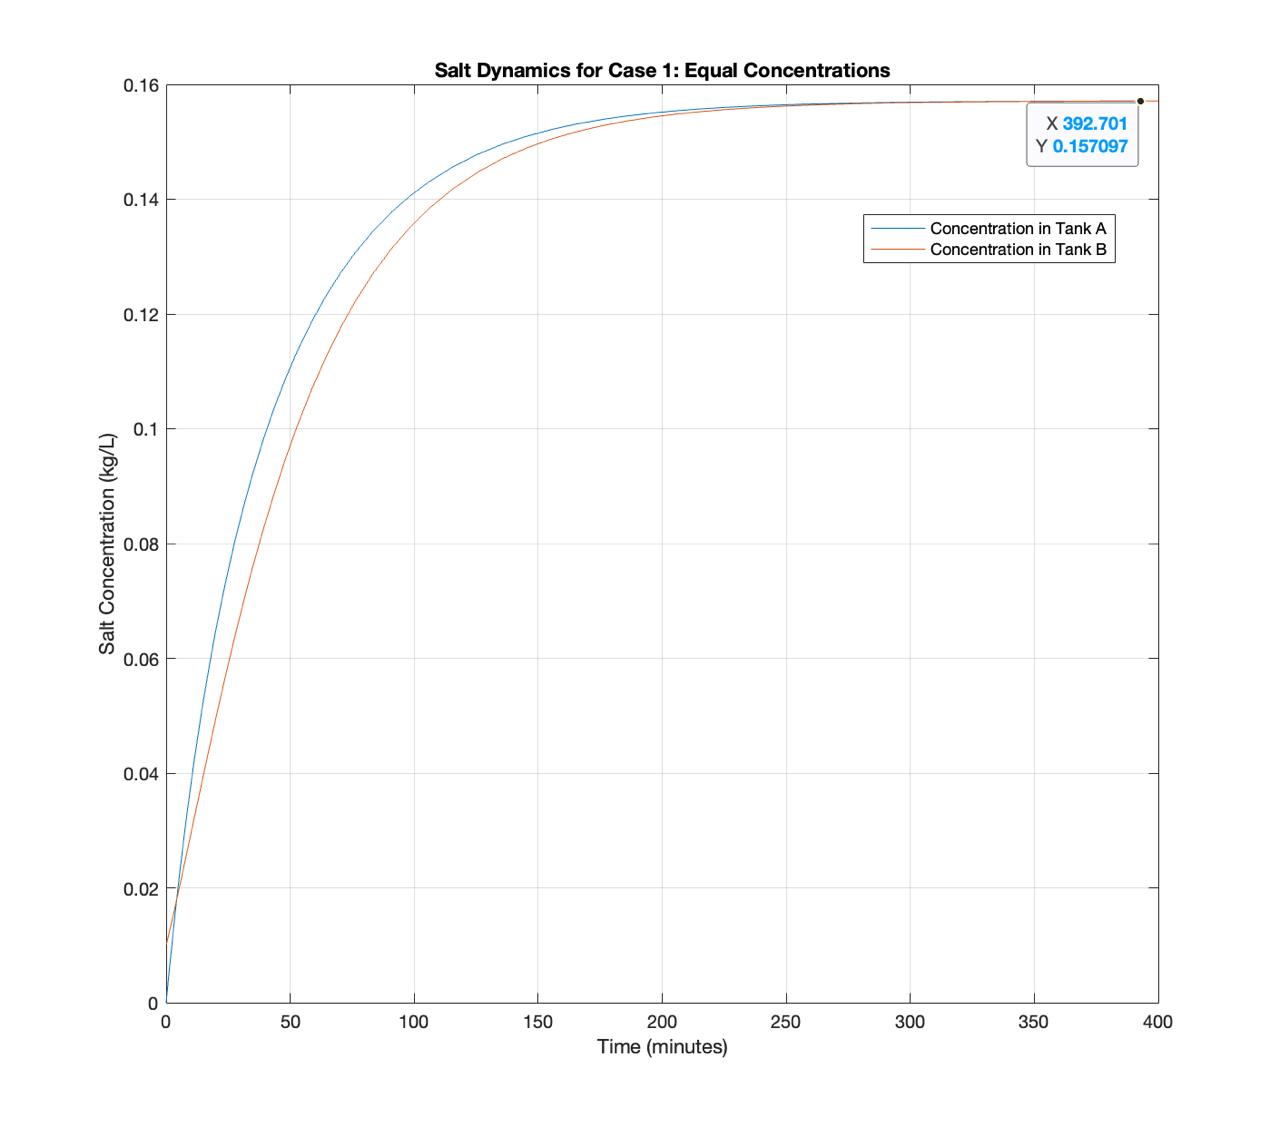
\includegraphics[width=0.75\linewidth,height=\textheight,keepaspectratio]{./eq_conc.jpg}
\caption{Evolution of salt concentration in Tanks A and B for Case
1.}\label{fig:eq_conc}
\end{figure}

\begin{figure}
\centering
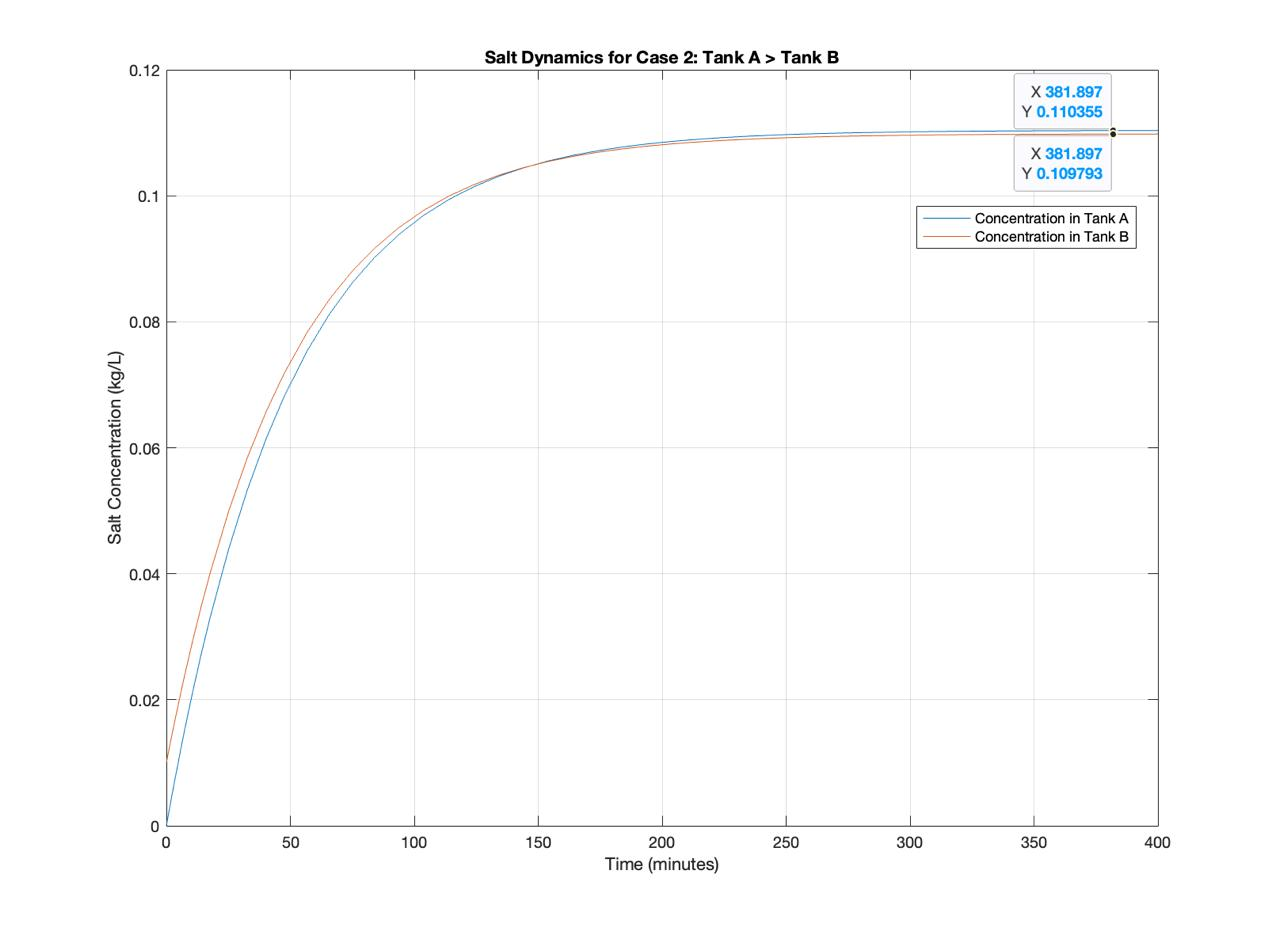
\includegraphics[width=0.75\linewidth,height=\textheight,keepaspectratio]{./gt_conc.jpg}
\caption{Evolution of salt concentration in Tanks A and B for Case
2.}\label{fig:gt_conc}
\end{figure}

A cursory glance at both figures would show that in both cases, the salt
concentrations converge to about the same values that the analytical
solution predicted. This, as well as the time evolution of both models,
will be investigated in the next chapter.

\section{Methods}\label{methods}

\section{Results}\label{results}

\section{Appendice}\label{appendice}

\subsection{Parameter search function}\label{sec:search_func}

\begin{Shaded}
\begin{Highlighting}[]
\KeywordTok{function} \VariableTok{params} \OperatorTok{=} \VariableTok{find\_params}\NormalTok{(}\VariableTok{comparator}\NormalTok{)}
\VariableTok{ks} \OperatorTok{=} \FloatTok{0.1}\OperatorTok{:}\FloatTok{0.02}\OperatorTok{:}\FloatTok{0.5}\OperatorTok{;}
\VariableTok{vs} \OperatorTok{=} \FloatTok{2}\OperatorTok{:}\FloatTok{0.05}\OperatorTok{:}\FloatTok{3}\OperatorTok{;}

\VariableTok{N} \OperatorTok{=} \VariableTok{numel}\NormalTok{(}\VariableTok{vs}\NormalTok{) }\OperatorTok{*} \FloatTok{4}\OperatorTok{;}
\VariableTok{i} \OperatorTok{=} \FloatTok{1}\OperatorTok{;}
\VariableTok{rates} \OperatorTok{=} \VariableTok{zeros}\NormalTok{(}\VariableTok{N}\OperatorTok{,}\FloatTok{4}\NormalTok{)}\OperatorTok{;}
\VariableTok{stop} \OperatorTok{=} \FloatTok{0}\OperatorTok{;}
\KeywordTok{for} \VariableTok{v\_ap} \OperatorTok{=} \VariableTok{vs}
    \KeywordTok{for} \VariableTok{v\_bp} \OperatorTok{=} \VariableTok{vs}
        \KeywordTok{for} \VariableTok{v\_am} \OperatorTok{=} \VariableTok{vs}
            \KeywordTok{for} \VariableTok{v\_bm} \OperatorTok{=} \VariableTok{vs}
                \KeywordTok{if}\NormalTok{ (}\VariableTok{v\_ap} \OperatorTok{+} \VariableTok{v\_bp}\NormalTok{) }\OperatorTok{==}\NormalTok{ (}\VariableTok{v\_am} \OperatorTok{+} \VariableTok{v\_bm}\NormalTok{)}
                    \VariableTok{rates}\NormalTok{(}\VariableTok{i}\OperatorTok{,}\FloatTok{1}\OperatorTok{:}\FloatTok{4}\NormalTok{) }\OperatorTok{=}\NormalTok{ [}\VariableTok{v\_ap}\OperatorTok{,} \VariableTok{v\_am}\OperatorTok{,} \VariableTok{v\_bp}\OperatorTok{,} \VariableTok{v\_bm}\NormalTok{]}\OperatorTok{;}
                    \VariableTok{i} \OperatorTok{=} \VariableTok{i} \OperatorTok{+} \FloatTok{1}\OperatorTok{;}
                    \KeywordTok{if} \VariableTok{i} \OperatorTok{\textgreater{}} \VariableTok{N}
                        \VariableTok{stop} \OperatorTok{=} \FloatTok{1}\OperatorTok{;}
                        \KeywordTok{break}\OperatorTok{;}
                    \KeywordTok{end}
                \KeywordTok{end}
            \KeywordTok{end}
            \KeywordTok{if} \VariableTok{stop} \OperatorTok{==} \FloatTok{1}
                \KeywordTok{break}\OperatorTok{;}
            \KeywordTok{end}
        \KeywordTok{end}
        \KeywordTok{if} \VariableTok{stop} \OperatorTok{==} \FloatTok{1}
            \KeywordTok{break}\OperatorTok{;}
        \KeywordTok{end}
    \KeywordTok{end}
    \KeywordTok{if} \VariableTok{stop} \OperatorTok{==} \FloatTok{1}
        \KeywordTok{break}
    \KeywordTok{end}
\KeywordTok{end}

\KeywordTok{for} \VariableTok{i} \OperatorTok{=} \FloatTok{1}\OperatorTok{:}\VariableTok{N}
  \VariableTok{v\_ap} \OperatorTok{=} \VariableTok{rates}\NormalTok{(}\VariableTok{i}\OperatorTok{,} \FloatTok{1}\NormalTok{)}\OperatorTok{;}
  \VariableTok{v\_am} \OperatorTok{=} \VariableTok{rates}\NormalTok{(}\VariableTok{i}\OperatorTok{,} \FloatTok{2}\NormalTok{)}\OperatorTok{;}
  \VariableTok{v\_bp} \OperatorTok{=} \VariableTok{rates}\NormalTok{(}\VariableTok{i}\OperatorTok{,} \FloatTok{3}\NormalTok{)}\OperatorTok{;}
  \VariableTok{v\_bm} \OperatorTok{=} \VariableTok{rates}\NormalTok{(}\VariableTok{i}\OperatorTok{,} \FloatTok{4}\NormalTok{)}\OperatorTok{;}

  \KeywordTok{for} \VariableTok{ka} \OperatorTok{=} \VariableTok{ks}
    \KeywordTok{for} \VariableTok{kb} \OperatorTok{=} \VariableTok{ks}
      \KeywordTok{for} \VariableTok{v\_ab} \OperatorTok{=} \VariableTok{vs}
        \KeywordTok{for} \VariableTok{v\_ba} \OperatorTok{=} \VariableTok{vs}
          \VariableTok{lhs} \OperatorTok{=}\NormalTok{ (}\VariableTok{ka}\OperatorTok{*}\VariableTok{v\_ap}\NormalTok{) }\OperatorTok{/}\NormalTok{ (}\VariableTok{kb}\OperatorTok{*}\VariableTok{v\_bp}\NormalTok{)}\OperatorTok{;}
          \VariableTok{rhs} \OperatorTok{=}\NormalTok{ (}\VariableTok{v\_ab} \OperatorTok{+} \VariableTok{v\_am} \OperatorTok{{-}} \VariableTok{v\_ba}\NormalTok{) }\OperatorTok{/}\NormalTok{ (}\VariableTok{v\_ba} \OperatorTok{+} \VariableTok{v\_bm} \OperatorTok{{-}} \VariableTok{v\_ab}\NormalTok{)}\OperatorTok{;}
          \VariableTok{is\_interesting} \OperatorTok{=} \VariableTok{v\_ap} \OperatorTok{\textasciitilde{}=} \VariableTok{v\_am} \OperatorTok{\&\&} \VariableTok{v\_ab} \OperatorTok{\textasciitilde{}=} \VariableTok{v\_ba} \OperatorTok{\&\&} \VariableTok{ka} \OperatorTok{\textasciitilde{}=} \VariableTok{kb}\OperatorTok{;}
            
          \KeywordTok{if} \VariableTok{comparator}\NormalTok{(}\VariableTok{lhs}\OperatorTok{,}\VariableTok{rhs}\NormalTok{) }\OperatorTok{\&\&} \VariableTok{is\_interesting}
            \VariableTok{params} \OperatorTok{=}\NormalTok{ [}\VariableTok{v\_ap}\OperatorTok{,} \VariableTok{v\_am}\OperatorTok{,} \VariableTok{v\_bp}\OperatorTok{,} \VariableTok{v\_bm}\OperatorTok{,} \VariableTok{ka}\OperatorTok{,} \VariableTok{kb}\OperatorTok{,} \VariableTok{v\_ab}\OperatorTok{,} \VariableTok{v\_ba}\NormalTok{]}\OperatorTok{\textquotesingle{};}
            \KeywordTok{return}
          \KeywordTok{end}
        \KeywordTok{end}
      \KeywordTok{end}
    \KeywordTok{end}
  \KeywordTok{end}
\KeywordTok{end}
\KeywordTok{end}
\end{Highlighting}
\end{Shaded}

\subsection{Numerical solution functions}\label{sec:numerical_func}

\begin{Shaded}
\begin{Highlighting}[]
\KeywordTok{function}\NormalTok{ [}\VariableTok{t}\OperatorTok{,} \VariableTok{c}\NormalTok{] }\OperatorTok{=} \VariableTok{numerical\_solution}\NormalTok{(}\VariableTok{params}\NormalTok{)}
  \VariableTok{V\_Ap} \OperatorTok{=} \VariableTok{params}\NormalTok{(}\FloatTok{1}\NormalTok{)}\OperatorTok{;} \VariableTok{V\_Am} \OperatorTok{=} \VariableTok{params}\NormalTok{(}\FloatTok{2}\NormalTok{)}\OperatorTok{;} \VariableTok{V\_Bp} \OperatorTok{=} \VariableTok{params}\NormalTok{(}\FloatTok{3}\NormalTok{)}\OperatorTok{;} \VariableTok{V\_Bm} \OperatorTok{=} \VariableTok{params}\NormalTok{(}\FloatTok{4}\NormalTok{)}\OperatorTok{;}
  \VariableTok{K\_A} \OperatorTok{=} \VariableTok{params}\NormalTok{(}\FloatTok{5}\NormalTok{)}\OperatorTok{;} \VariableTok{K\_B} \OperatorTok{=} \VariableTok{params}\NormalTok{(}\FloatTok{6}\NormalTok{)}\OperatorTok{;} \VariableTok{V\_AB} \OperatorTok{=} \VariableTok{params}\NormalTok{(}\FloatTok{7}\NormalTok{)}\OperatorTok{;} \VariableTok{V\_BA} \OperatorTok{=} \VariableTok{params}\NormalTok{(}\FloatTok{8}\NormalTok{)}\OperatorTok{;} 

  \CommentTok{\% Time span}
  \VariableTok{tspan} \OperatorTok{=}\NormalTok{ [}\FloatTok{0}\OperatorTok{,} \FloatTok{400}\NormalTok{]}\OperatorTok{;}
  
  \CommentTok{\% Initial conditions}
  \VariableTok{x0} \OperatorTok{=}\NormalTok{ [}\FloatTok{0}\OperatorTok{;} \FloatTok{1}\NormalTok{]}\OperatorTok{;}
  
  \CommentTok{\% Solve ODE}
\NormalTok{  [}\VariableTok{t}\OperatorTok{,} \VariableTok{x}\NormalTok{] }\OperatorTok{=} \VariableTok{ode45}\NormalTok{(}\OperatorTok{@}\NormalTok{(}\VariableTok{t}\OperatorTok{,} \VariableTok{x}\NormalTok{) }\VariableTok{salt\_dynamics}\NormalTok{(}\VariableTok{t}\OperatorTok{,} \VariableTok{x}\OperatorTok{,} \VariableTok{V\_Ap}\OperatorTok{,} \VariableTok{V\_Am}\OperatorTok{,} \VariableTok{V\_Bp}\OperatorTok{,} \OperatorTok{...}
        \VariableTok{V\_Bm}\OperatorTok{,} \VariableTok{V\_AB}\OperatorTok{,} \VariableTok{V\_BA}\OperatorTok{,} \VariableTok{K\_A}\OperatorTok{,} \VariableTok{K\_B}\NormalTok{)}\OperatorTok{,} \VariableTok{tspan}\OperatorTok{,} \VariableTok{x0}\NormalTok{)}\OperatorTok{;}

  \CommentTok{\% Convert salt amounts to concentrations}
  \VariableTok{c} \OperatorTok{=} \VariableTok{S} \OperatorTok{/} \FloatTok{100}\OperatorTok{;}
\KeywordTok{end}

\KeywordTok{function} \VariableTok{dxdt} \OperatorTok{=} \VariableTok{salt\_dynamics}\NormalTok{(}\OperatorTok{\textasciitilde{},} \VariableTok{x}\OperatorTok{,} \VariableTok{V\_Ap}\OperatorTok{,} \VariableTok{V\_Am}\OperatorTok{,} \VariableTok{V\_Bp}\OperatorTok{,} \VariableTok{V\_Bm}\OperatorTok{,} \VariableTok{V\_AB}\OperatorTok{,} \VariableTok{V\_BA}\OperatorTok{,} \VariableTok{K\_A}\OperatorTok{,} \VariableTok{K\_B}\NormalTok{)}
  \VariableTok{x\_A} \OperatorTok{=} \VariableTok{x}\NormalTok{(}\FloatTok{1}\NormalTok{)}\OperatorTok{;} \CommentTok{\% Salt in Tank A}
  \VariableTok{x\_B} \OperatorTok{=} \VariableTok{x}\NormalTok{(}\FloatTok{2}\NormalTok{)}\OperatorTok{;} \CommentTok{\% Salt in Tank B}
  
  \CommentTok{\% Tank A}
  \VariableTok{dx\_A} \OperatorTok{=} \VariableTok{V\_Ap} \OperatorTok{*} \VariableTok{K\_A} \OperatorTok{{-}} \VariableTok{V\_Am} \OperatorTok{*} \VariableTok{x\_A} \OperatorTok{/} \FloatTok{100} \OperatorTok{{-}} \VariableTok{V\_AB} \OperatorTok{*} \VariableTok{x\_A} \OperatorTok{/} \FloatTok{100} \OperatorTok{+} \VariableTok{V\_BA} \OperatorTok{*} \VariableTok{x\_B} \OperatorTok{/} \FloatTok{100}\OperatorTok{;}
  
  \CommentTok{\% Tank B}
  \VariableTok{dx\_B} \OperatorTok{=} \VariableTok{V\_Bp} \OperatorTok{*} \VariableTok{K\_B} \OperatorTok{{-}} \VariableTok{V\_Bm} \OperatorTok{*} \VariableTok{x\_B} \OperatorTok{/} \FloatTok{100} \OperatorTok{{-}} \VariableTok{V\_BA} \OperatorTok{*} \VariableTok{x\_B} \OperatorTok{/} \FloatTok{100} \OperatorTok{+} \VariableTok{V\_AB} \OperatorTok{*} \VariableTok{x\_A} \OperatorTok{/} \FloatTok{100}\OperatorTok{;}
  
  \VariableTok{dxdt} \OperatorTok{=}\NormalTok{ [}\VariableTok{dx\_A}\OperatorTok{;} \VariableTok{dx\_B}\NormalTok{]}\OperatorTok{;}
\KeywordTok{end}
\end{Highlighting}
\end{Shaded}

\section{Summary}\label{summary}
